\chapter{Experiment Results}

\section{Introduction}
This chapter presents the results from performing the experiments. The characteristics of the dataset are summarized on the exploratory data analysis section. The last section compares PRFR and REINFORCE in terms of their effectiveness in training an AS model for solving subgraph isomorphism problems.

\section{Exploratory Data Analysis}
\subsection{Data Summary}

The following statistical measures were taken for the results of each feature and algorithm:

\begin{itemize}
	\item \textbf{min} - minimum
	\item \textbf{qu\_-1st} - 25\% quantile
	\item \textbf{med} - median
	\item \textbf{mean} -  arithmetic mean
	\item \textbf{qu\_3rd} - 75\%-quantile
	\item \textbf{max} - maximum
	\item \textbf{sd} - standard deviation
	\item \textbf{coeff\_var} - coefficient of variation (standard deviation / arithmetic mean)
\end{itemize}

\begin{table}[H]
	\centering
	\resizebox{\columnwidth}{!}{%
	\begin{tabular}{|l|r|r|r|r|r|r|r|r|}
		\hline
		\multicolumn{1}{|c|}{\textbf{Features}} & \multicolumn{1}{c|}{\textbf{min}} & \multicolumn{1}{c|}{\textbf{qu\_1st}} & \multicolumn{1}{c|}{\textbf{med}} & \multicolumn{1}{c|}{\textbf{mean}} & \multicolumn{1}{c|}{\textbf{qu\_3rd}} & \multicolumn{1}{c|}{\textbf{max}} & \multicolumn{1}{c|}{\textbf{sd}} & \multicolumn{1}{c|}{\textbf{coeff\_var}} \\ \hline
		cheap.pattern.time                      & 0.0000                            & 0.0000                                & 0.0000                            & 0.0035                             & 0.0000                                & 1.0000                            & 0.0590                           & 16.8908                                  \\ \hline
		cheap.pattern.vertices                  & 4.0000                            & 48.0000                               & 80.0000                           & 109.3787                           & 128.0000                              & 900.0000                          & 114.9942                         & 1.0513                                   \\ \hline
		cheap.pattern.edges                     & 4.0000                            & 112.0000                              & 240.0000                          & 598.8704                           & 696.0000                              & 12410.0000                        & 1073.5139                        & 1.7926                                   \\ \hline
		cheap.pattern.loops                     & 0.0000                            & 0.0000                                & 0.0000                            & 0.2451                             & 0.0000                                & 9.0000                            & 1.3121                           & 5.3543                                   \\ \hline
		cheap.pattern.meandeg                   & 1.7867                            & 3.6364                                & 5.4286                            & 10.4274                            & 10.0000                               & 99.0000                           & 14.4378                          & 1.3846                                   \\ \hline
		cheap.pattern.maxdeg                    & 2.0000                            & 8.0000                                & 11.0000                           & 20.6091                            & 26.0000                               & 269.0000                          & 27.3313                          & 1.3262                                   \\ \hline
		cheap.pattern.degisfixed                & 0.0000                            & 0.0000                                & 0.0000                            & 0.1132                             & 0.0000                                & 1.0000                            & 0.3168                           & 2.7993                                   \\ \hline
		cheap.pattern.density                   & 0.0045                            & 0.0441                                & 0.0978                            & 0.1683                             & 0.1830                                & 1.0000                            & 0.2194                           & 1.3038                                   \\ \hline
		cheap.target.time                       & 0.0000                            & 0.0000                                & 0.0000                            & 3.9988                             & 2.0000                                & 55.0000                           & 9.5821                           & 2.3963                                   \\ \hline
		cheap.target.vertices                   & 10.0000                           & 216.0000                              & 561.0000                          & 1147.3385                          & 1430.0000                             & 6671.0000                         & 1440.1846                        & 1.2552                                   \\ \hline
		cheap.target.edges                      & 15.0000                           & 930.0000                              & 2074.0000                         & 7176.6114                          & 5994.0000                             & 209000.0000                       & 21594.1676                       & 3.0090                                   \\ \hline
		cheap.target.loops                      & 0.0000                            & 0.0000                                & 0.0000                            & 1.6306                             & 0.0000                                & 144.0000                          & 13.3146                          & 8.1656                                   \\ \hline
		cheap.target.meandeg                    & 0.4357                            & 4.1983                                & 6.0000                            & 19.4312                            & 11.9172                               & 270.6950                          & 39.8146                          & 2.0490                                   \\ \hline
		cheap.target.maxdeg                     & 2.0000                            & 10.0000                               & 19.0000                           & 102.2134                           & 52.0000                               & 4973.0000                         & 384.0174                         & 3.7570                                   \\ \hline
		cheap.target.degisfixed                 & 0.0000                            & 0.0000                                & 0.0000                            & 0.1492                             & 0.0000                                & 1.0000                            & 0.3563                           & 2.3885                                   \\ \hline
		cheap.target.density                    & 0.0005                            & 0.0030                                & 0.0119                            & 0.0729                             & 0.0588                                & 1.0000                            & 0.1585                           & 2.1736                                   \\ \hline
		distance.pattern.time                   & 0.0000                            & 0.0000                                & 0.0000                            & 2.0349                             & 1.0000                                & 93.0000                           & 8.0467                           & 3.9543                                   \\ \hline
		distance.pattern.isconnected            & 0.0000                            & 1.0000                                & 1.0000                            & 0.7976                             & 1.0000                                & 1.0000                            & 0.4019                           & 0.5039                                   \\ \hline
		distance.pattern.meandistance           & 1.0000                            & 2.0010                                & 2.7778                            & 3.9349                             & 4.1227                                & 80.6687                           & 5.6418                           & 1.4338                                   \\ \hline
		distance.pattern.maxdistance            & 1.0000                            & 3.0000                                & 5.0000                            & 8.9328                             & 9.0000                                & 240.0000                          & 16.9947                          & 1.9025                                   \\ \hline
		distance.pattern.proportiondistancege2  & 0.0000                            & 0.6000                                & 0.8466                            & 0.7406                             & 0.9319                                & 0.9929                            & 0.2661                           & 0.3593                                   \\ \hline
		distance.pattern.proportiondistancege3  & 0.0000                            & 0.0974                                & 0.5000                            & 0.4605                             & 0.8237                                & 0.9834                            & 0.3507                           & 0.7615                                   \\ \hline
		distance.pattern.proportiondistancege4  & 0.0000                            & 0.0000                                & 0.1957                            & 0.3091                             & 0.6094                                & 0.9752                            & 0.3225                           & 1.0432                                   \\ \hline
		distance.target.time                    & 0.0000                            & 5.0000                                & 32.0000                           & 553.0529                           & 208.0000                              & 9962.0000                         & 1474.8373                        & 2.6667                                   \\ \hline
		distance.target.isconnected             & 0.0000                            & 0.0000                                & 1.0000                            & 0.7095                             & 1.0000                                & 1.0000                            & 0.4540                           & 0.6399                                   \\ \hline
		distance.target.meandistance            & 1.0000                            & 2.4484                                & 3.7010                            & 7.4919                             & 7.1508                                & 100.6250                          & 11.7237                          & 1.5648                                   \\ \hline
		distance.target.maxdistance             & 1.0000                            & 5.0000                                & 8.0000                            & 16.3768                            & 16.0000                               & 200.0000                          & 24.8081                          & 1.5148                                   \\ \hline
		distance.target.proportiondistancege2   & 0.0000                            & 0.6082                                & 0.9502                            & 0.7944                             & 0.9900                                & 0.9993                            & 0.2896                           & 0.3645                                   \\ \hline
		distance.target.proportiondistancege3   & 0.0000                            & 0.2472                                & 0.7260                            & 0.5990                             & 0.9502                                & 0.9985                            & 0.3708                           & 0.6190                                   \\ \hline
		distance.target.proportiondistancege4   & 0.0000                            & 0.0288                                & 0.3875                            & 0.4514                             & 0.8813                                & 0.9973                            & 0.3838                           & 0.8502                                   \\ \hline
		lad.values.removed                      & 0.0000                            & 0.0000                                & 0.0000                            & 28733.8725                         & 10673.0000                            & 844304.0000                       & 81827.2598                       & 2.8478                                   \\ \hline
		lad.values.removed.percent              & 0.0000                            & 2.3503                                & 49.2371                           & 51.7472                            & 100.0000                              & 100.0000                          & 41.8261                          & 0.8083                                   \\ \hline
		lad.values.removed.min                  & 0.0000                            & 0.0000                                & 0.0000                            & 6.7000                             & 0.3190                                & 99.9700                           & 19.4023                          & 2.8959                                   \\ \hline
		lad.values.removed.max                  & 0.0000                            & 0.0000                                & 0.0000                            & 33.1602                            & 88.2143                               & 99.9816                           & 42.8695                          & 1.2928                                   \\ \hline
		lad.time                                & 0.0000                            & 0.0000                                & 0.0000                            & 7.1210                             & 3.0000                                & 3964.0000                         & 80.7295                          & 11.3367                                  \\ \hline
	\end{tabular}%
}
\caption{Summary of features}
\label{tbl:featuresummary}
\end{table}

\begin{table}[H]
	\centering
	\resizebox{\columnwidth}{!}{%
		\begin{tabular}{|l|r|r|r|r|r|r|r|r|}
			\hline
			\multicolumn{1}{|c|}{\textbf{Algorithm}} & \multicolumn{1}{c|}{\textbf{min}} & \multicolumn{1}{c|}{\textbf{qu\_1st}} & \multicolumn{1}{c|}{\textbf{med}} & \multicolumn{1}{c|}{\textbf{mean}} & \multicolumn{1}{c|}{\textbf{qu\_3rd}} & \multicolumn{1}{c|}{\textbf{max}} & \multicolumn{1}{c|}{\textbf{sd}} & \multicolumn{1}{c|}{\textbf{coeff\_var}} \\ \hline
			lad                                      & 0                                 & 3                                     & 33                                & 5935035.15                         & 1214                                  & 1.00E+08                          & 22874350.97                      & 3.8541                                   \\ \hline
			supplementallad                          & 0                                 & 3                                     & 22                                & 4841120.76                         & 402                                   & 1.00E+08                          & 20810140.52                      & 4.2986                                   \\ \hline
			vf2                                      & 0                                 & 6                                     & 115                               & 27565110.75                        & 1.00E+08                              & 1.00E+08                          & 44243664.13                      & 1.6051                                   \\ \hline
			glasgow1                                 & 0                                 & 4                                     & 25                                & 4158094.27                         & 199                                   & 1.00E+08                          & 19437830.22                      & 4.6747                                   \\ \hline
			glasgow2                                 & 0                                 & 12                                    & 61                                & 3196878.81                         & 414                                   & 1.00E+08                          & 17126177.54                      & 5.3572                                   \\ \hline
			glasgow3                                 & 0                                 & 33                                    & 168                               & 3212027.69                         & 1072                                  & 1.00E+08                          & 17153623.91                      & 5.3404                                   \\ \hline
			glasgow4                                 & 0                                 & 113                                   & 478                               & 4333647.25                         & 7178                                  & 1.00E+08                          & 19233485.20                      & 4.4382                                   \\ \hline
		\end{tabular}%
	}
	\caption[Summary of algorithms]{Summary of algorithms. All values represent runtime in milliseconds.}
	\label{tbl:algosummary}
\end{table}

\subsection{Distributions}
Histograms for features and algorithm runtimes are displayed in the following plots. The red dashed lines denote the median of the distribution.

\begin{figure}[H]
	\centering
	\scalebox{.65}{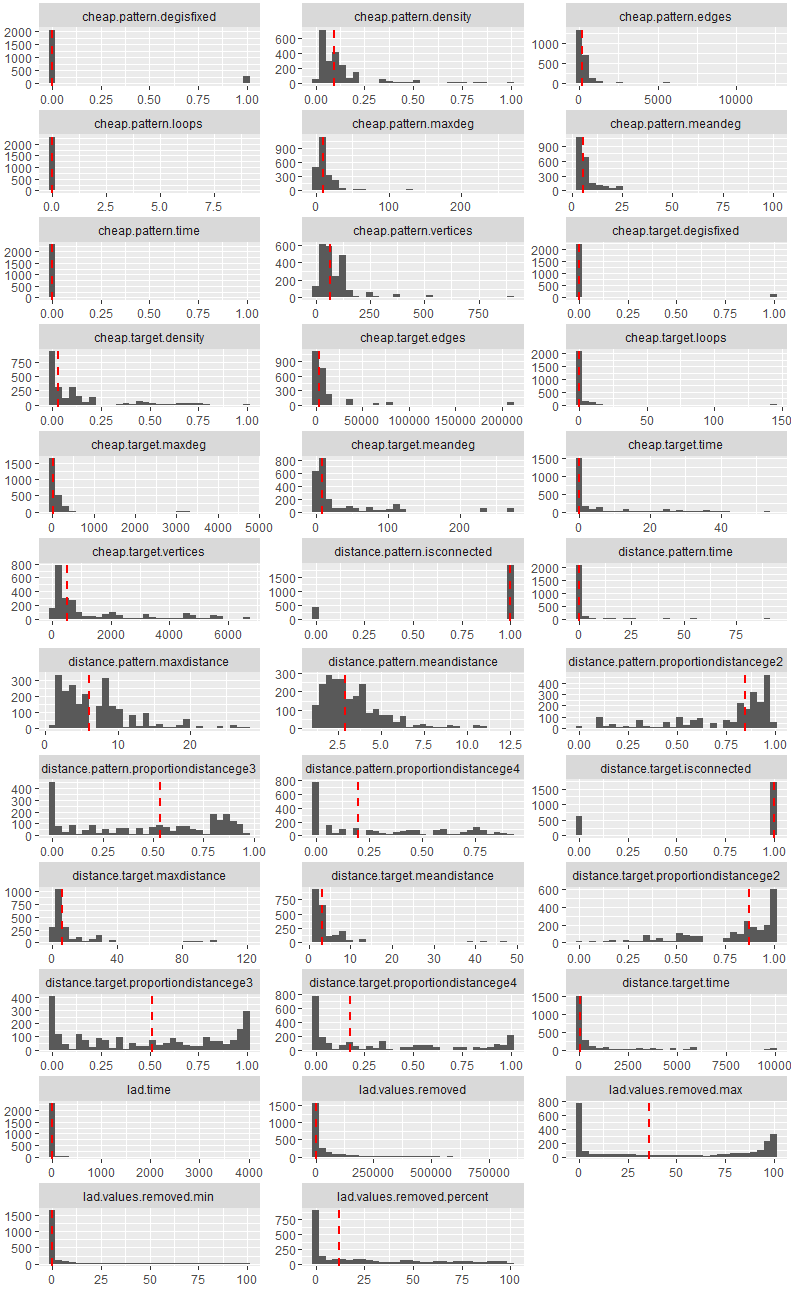
\includegraphics{./img/featuredist.png}}
	\caption{Feature distributions}
	\label{fig:featuredist}
\end{figure}

\begin{figure}[H]
	\centering
	\scalebox{.55}{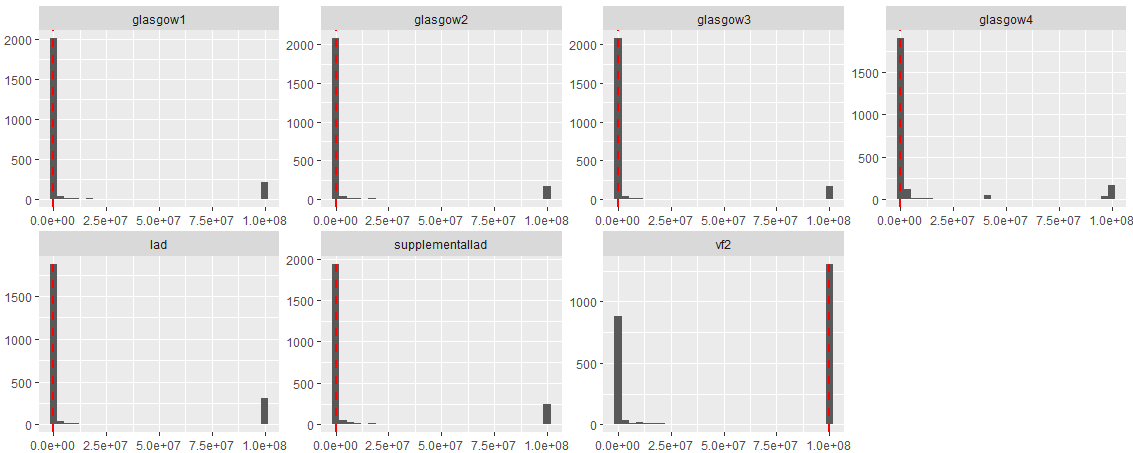
\includegraphics{./img/algodist.png}}
	\caption{Algorithm distributions}
	\label{fig:algodist}
\end{figure}

\begin{figure}[H]
	\centering
	\scalebox{.55}{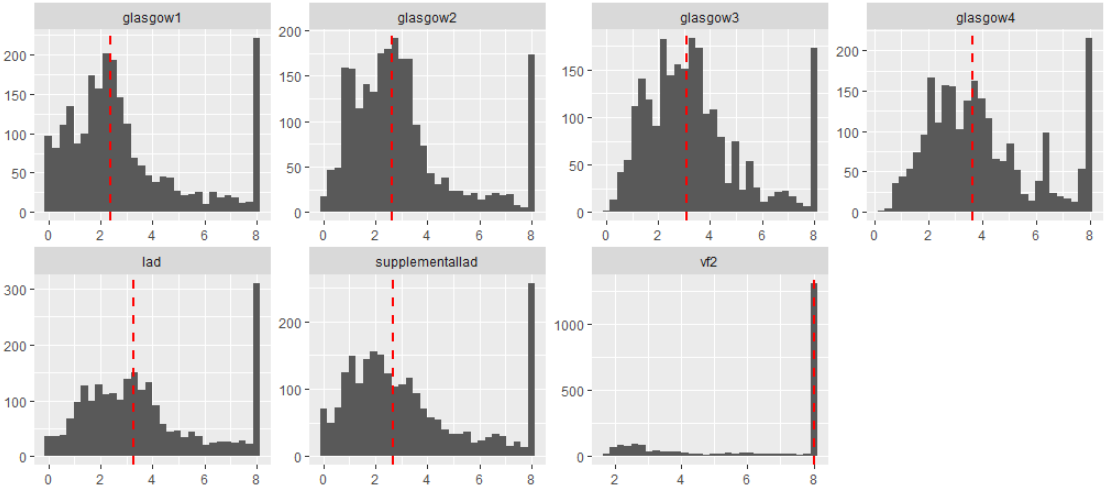
\includegraphics{./img/logalgodist.png}}
	\caption{Log-scaled algorithm distributions}
	\label{fig:logalgodist}
\end{figure}

\section{AS Model Performance Evaluation}

The mean MCP of the AS model trained using REINFORCE is 4x worse than one trained using PRFR. REINFORCE is not able to surpass the performance standard set by PORTSUB, which was hoped to be surpassed in this study.

\begin{table}[H]
	\begin{tabular}{|l|l|l|l|l|}
		\hline
		\textbf{AS Model} & \textbf{Mean MCP} & \textbf{\# Solved problems} & \textbf{Mean Performance} & \textbf{Median Performance} \\ \hline
		VBS               & 0.0               & 2,219                       & 5,822,809.0               & 79.0                        \\ \hline
		PRFR              & 621,662.5         & 2,208                       & 6,446,129.0               & 1,748.5                     \\ \hline
		SBS               & 1,963,498.6       & 2,173                       & 7,786,308.0               & 539.0                       \\ \hline
		REINFORCE         & 2,318,832.0       & 2,156                       & 8,168,306.0               & 929.0                       \\ \hline
	\end{tabular}
	\caption{AS model performance evaluation results}
	\label{tbl:asresults}
\end{table}

Despite REINFORCE failing to obtain better MCP than PRFR, it showed improvement on median performance, reporting almost 2x better than PRFR.  Its significance becomes clearer by analyzing the cumulative density function (CDF) plot which visualizes the distribution of runtimes of the selected algorithms on all problems, as illustrated Figure \ref{fig:cdf}.  REINFORCE is able to select more optimal algorithms than PRFR on the easier problems (solvable within $10-10^4$ ms) on the dataset. For difficult problems which are solvable within at least 105-108 ms, REINFORCE selected worse-performing algorithms than PRFR. Although the easier problems constitute the majority (75\%) of the dataset, its influence on the mean MCP is much lesser than the harder problems. REINFORCE performed better than PRFR in solving the easy problems, but underperformed when it came to solving the more difficult problems. 

\begin{figure}[H]	
	\centering
	\scalebox{.9}{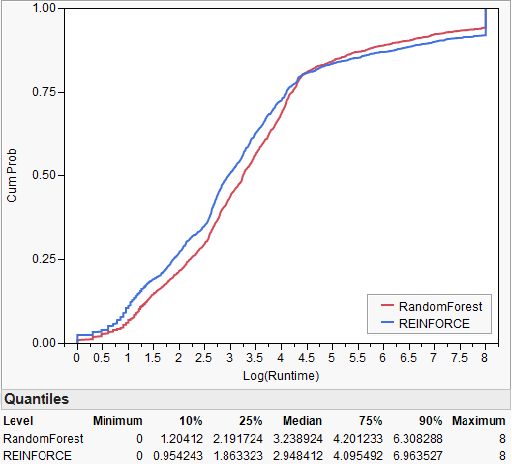
\includegraphics{./img/cdf.png}}
	\caption{Cumulative density plot of AS model performance}
	\label{fig:cdf}
\end{figure}